\documentclass[14pt,t,dvipsnames]{beamer}
% \setbeamerfont{alerted text}{series=\bfseries\large}
\setbeamertemplate{navigation symbols}{}
\usefonttheme[onlymath]{serif}

\setlength{\parskip}{1em}


\usepackage[utf8]{inputenc}
\usepackage[T1]{fontenc}
\usepackage{lmodern}
\usepackage{makecell} %...used in tabular for \thead
 
%...For highlighting
\usepackage{xcolor, soul} 
\makeatletter
\let\HL\hl
\renewcommand\hl{%
  \let\set@color\beamerorig@set@color
  \let\reset@color\beamerorig@reset@color
  \HL}
\makeatother

\hypersetup{
    colorlinks=true,
    linkcolor=blue,
    filecolor=magenta,      
    urlcolor=cyan,
    pdftitle={Overleaf Example},
    pdfpagemode=FullScreen,
}

\usepackage[acronym]{glossaries}
\glsdisablehyper %...disables hyperlinks for glossary terms in frames


\usepackage{amsmath}  %...for the equation* environment

%...Tikz and PGF packages
\usepackage{tikz}
\usetikzlibrary{calc,math}
\usetikzlibrary{patterns}
\usepackage{tikz-cd}
\usepackage{pgfplots}
\pgfplotsset{compat=1.18}
\usetikzlibrary{backgrounds} %...For shading portions of graphs
% \usetikzlibrary{math}
\tikzset{>=latex} %...For pretty arrows
\tikzset{
    declare function = {trajectoryequationTEN(\x,\vi,\thetai)= tan(\thetai)*\x - 10*\x^2/(2*(\vi*cos(\thetai))^2);},
    declare function = {trajectoryequation(\x,\vi,\thetai)= tan(\thetai)*\x - 9.8*\x^2/(2*(\vi*cos(\thetai))^2);},
    declare function = {patheq(\x,\yi,\vi,\thetai)= \yi + tan(\thetai)*\x - 9.8*\x^2/(2*(\vi*cos(\thetai))^2);}
} %...Plots the trajectory equation for projectile motion:


\usetikzlibrary{positioning}
\tikzset{onslide/.code args={<#1>#2}{%
  \only<#1>{\pgfkeysalso{#2}} % \pgfkeysalso doesn't change the path
}}

%...SI Units
\usepackage{siunitx}
%\sisetup{per-mode=fraction}
\usepackage{cancel}
\DeclareSIUnit{\mile}{mi}


%...Symbols packages
\usepackage{fontawesome} % for \faHome
\usepackage{tikzsymbols} % for tree and stick figure
\usepackage{twemojis} %...for twitter emojis
\usepackage{utfsym}  %...for a basic star symbol

%...Breaks long URLs
\usepackage{xurl}

%...Multiple columns for table of contents
\usepackage{multicol}

%...beamer specific
\AtBeginSection[]
{
  \begin{frame}
    \frametitle{Table of Contents}
    \begin{multicols}{2}
        \tableofcontents[currentsection]
    \end{multicols}
  \end{frame}
}

\setbeamerfont{frametitle}{size=\normalsize}

%...Vector commands
\newcommand{\bvec}[1]{\vec{\mathbf{#1}}}
\newcommand{\bhat}[1]{\,\hat{\mathbf{#1}}}


%%%%%%% DST, XVT, and VAT Triangles
\newcommand{\DSTtriangle}[1][]{%
    % Key-value setup for the shade argument
    \pgfkeys{/DST/.cd, shade/.store in=\DSTshade, shade=none, #1}%
    
    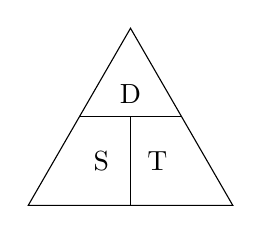
\begin{tikzpicture}[x=1.5cm,y=1.5cm]
        \coordinate (D) at (0,1);
        \coordinate (S) at ({cos(210)},{sin(210)});
        \coordinate (T) at ({cos(330)},{sin(330)});
        
        % Midpoints
        \coordinate (M1) at ($(D)!0.5!(S)$);
        \coordinate (M2) at ($(D)!0.5!(T)$);
        \coordinate (M3) at ($(M1)!0.5!(M2)$);
        \coordinate (M4) at ($(S)!0.5!(T)$);
        
        % Variables for comparison
        \def\shadeD{D}
        \def\shadeS{S}
        \def\shadeT{T}
        
        % Shading logic (drawn first so lines appear on top)
        \ifx\DSTshade\shadeD
            \fill[gray!30] (D) -- (M1) -- (M2) -- cycle;
        \fi
        \ifx\DSTshade\shadeS
            \fill[gray!30] (S) -- (M4) -- (M3) -- (M1) -- cycle;
        \fi
        \ifx\DSTshade\shadeT
            \fill[gray!30] (T) -- (M4) -- (M3) -- (M2) -- cycle;
        \fi
        
        % Triangle outer border
        \draw (D) -- (S) -- (T) -- cycle;
        
        % Lines between midpoints
        \draw (M1) -- (M2) node[pos=0.5,above=0.03] {D};
        \draw (M3) -- (M4) node[pos=0.5,left=0.1] {S} node[pos=0.5,right=0.06] {T};
    \end{tikzpicture}
}

\newcommand{\XVTtriangle}[1][]{%
    % Key-value setup for the shade argument
    \pgfkeys{/DST/.cd, shade/.store in=\DSTshade, shade=none, #1}%
    
    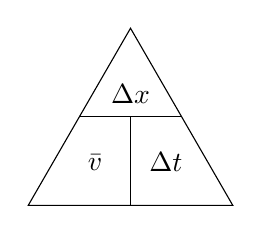
\begin{tikzpicture}[x=1.5cm,y=1.5cm]
        \coordinate (D) at (0,1);
        \coordinate (S) at ({cos(210)},{sin(210)});
        \coordinate (T) at ({cos(330)},{sin(330)});
        
        % Midpoints
        \coordinate (M1) at ($(D)!0.5!(S)$);
        \coordinate (M2) at ($(D)!0.5!(T)$);
        \coordinate (M3) at ($(M1)!0.5!(M2)$);
        \coordinate (M4) at ($(S)!0.5!(T)$);
        
        % Variables for comparison
        \def\shadeD{X}
        \def\shadeS{V}
        \def\shadeT{T}
        
        % Shading logic (drawn first so lines appear on top)
        \ifx\DSTshade\shadeD
            \fill[gray!30] (D) -- (M1) -- (M2) -- cycle;
        \fi
        \ifx\DSTshade\shadeS
            \fill[gray!30] (S) -- (M4) -- (M3) -- (M1) -- cycle;
        \fi
        \ifx\DSTshade\shadeT
            \fill[gray!30] (T) -- (M4) -- (M3) -- (M2) -- cycle;
        \fi
        
        % Triangle outer border
        \draw (D) -- (S) -- (T) -- cycle;
        
        % Lines between midpoints
        \draw (M1) -- (M2) node[pos=0.5,above=0.03] {$\Delta x$};
        \draw (M3) -- (M4) node[pos=0.5,shift={(-0.3,-0.01)}] {$\bar{v}$} node[pos=0.5,shift={(0.3,-0.01)}] {$\Delta t$};
    \end{tikzpicture}
}

\newcommand{\VATtriangle}[1][]{%
    % Key-value setup for the shade argument
    \pgfkeys{/DST/.cd, shade/.store in=\DSTshade, shade=none, #1}%
    
    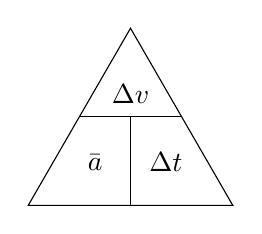
\begin{tikzpicture}[x=1.5cm,y=1.5cm]
        \coordinate (D) at (0,1);
        \coordinate (S) at ({cos(210)},{sin(210)});
        \coordinate (T) at ({cos(330)},{sin(330)});
        
        % Midpoints
        \coordinate (M1) at ($(D)!0.5!(S)$);
        \coordinate (M2) at ($(D)!0.5!(T)$);
        \coordinate (M3) at ($(M1)!0.5!(M2)$);
        \coordinate (M4) at ($(S)!0.5!(T)$);
        
        % Variables for comparison
        \def\shadeD{V}
        \def\shadeS{A}
        \def\shadeT{T}
        
        % Shading logic (drawn first so lines appear on top)
        \ifx\DSTshade\shadeD
            \fill[gray!30] (D) -- (M1) -- (M2) -- cycle;
        \fi
        \ifx\DSTshade\shadeS
            \fill[gray!30] (S) -- (M4) -- (M3) -- (M1) -- cycle;
        \fi
        \ifx\DSTshade\shadeT
            \fill[gray!30] (T) -- (M4) -- (M3) -- (M2) -- cycle;
        \fi
        
        % Triangle outer border
        \draw (D) -- (S) -- (T) -- cycle;
        
        % Lines between midpoints
        \draw (M1) -- (M2) node[pos=0.5,above=0.03] {$\Delta v$};
        \draw (M3) -- (M4) node[pos=0.5,shift={(-0.3,-0.01)}] {$\bar{a}$} node[pos=0.5,shift={(0.3,-0.01)}] {$\Delta t$};
    \end{tikzpicture}
}

%...Speedometer
\newcommand{\speedometer}[3]{%
    % #1: X-shift (y is fixed at 2) (e.g., 1)
    % #2: Needle rotation angle (e.g., 20)
    % #3: Top label (e.g., \texttt{Speed})
    % #4: Bottom readout (e.g., \textsf{32.0\,m/s})
    \begin{scope}[shift={#1},x=1.3cm,y=1.3cm]
        \draw (0,0) circle (1);
        \foreach \x in {340,360,...,560} {
            \coordinate (P) at ({cos(\x)},{sin(\x)});
            \draw[ultra thick,gray] (P) -- ($(P)!0.16!(0,0)$);
        }
        \foreach \x in {350,370,...,550} {
            \coordinate (P) at ({cos(\x)},{sin(\x)});
            \draw[thick,gray] (P) -- ($(P)!0.08!(0,0)$);
        }
        \fill (0,0) circle (0.02);
        \draw[fill=lightgray,rotate={#2},red] (0,0.02) rectangle (0.975,-0.02);
        \node at (0,0.4) {\texttt{Speed}};
        \draw[rounded corners] (-0.65,-0.75) rectangle ++(1.3,0.5) node[pos=0.5] {\textsf{#3\,m/s}};
    \end{scope}
}


%...UNIT 1: CONSTANT VELOCITY

\newcommand{\xygraphI}[3]{
\begin{tikzpicture}
    \begin{axis}[height=7.7cm,width=8.5cm,
        axis lines=center,
        ylabel={$y$},
        xlabel={$x$},
        ymin=-10,ymax=10,
        xmin=-10,xmax=10,
        ytick={-10,-8,...,10},
        xtick={-10,-8,...,10},
        grid=both, 
        minor y tick num=1,
        minor x tick num=1,
    ]
        \addplot[thick,domain=-10:10] {#1*x + #2};
        \ifprintanswers
            \addplot[red,only marks,mark=*] coordinates{#3};
        \fi
    \end{axis}
\end{tikzpicture}
}


\newcommand{\distancegraphI}[1]{
    \begin{tikzpicture}
        \begin{axis}[height=6.5cm,width=6.8cm,
            axis lines=left,
            xlabel = {Time (hours)},
            ylabel = {Distance (miles)},
            ymin=0, ymax=100,
            xmin=0, xmax=5,
            ytick={0,10,...,100},
            xtick={0,1,...,5},
            minor x tick num=1,
            grid=both,
            ]
            \addplot[very thick,domain=0:5] {#1*x};
        \end{axis}
    \end{tikzpicture}
}

\newcommand{\positiongraphI}[3]{
    \begin{tikzpicture}
        \begin{axis}[height=5.6cm,width=6.5cm,
            axis lines=left,
            xlabel = {Time (s)},
            ylabel = {Position (m)},
            ymin=0, ymax=20,
            xmin=0, xmax=14,
            ytick={0,4,...,20},
            xtick={0,2,...,14},
            minor y tick num=3,
            minor x tick num=1,
            grid=both,
            ]
            \addplot[very thick,domain=0:14] {#1*x + #2};
            \ifprintanswers
                \addplot[red,only marks,mark=*] coordinates{#3};
            \fi
        \end{axis}
    \end{tikzpicture}

%...AI-CHATBOT PROMPT:
% In an xy plane, the y limits are 0 to 20, and the x limits are 0 to 14. Give me 5 excellent linear equations (y = mx + b) for students to practice slope calculations. Output the results in the form \positiongraphI{m}{b}{coordinates} where coordinates should be in the form (x1,y1)(x2,y2), representing 2 points on the line for calculating slope. 
}

\newcommand{\positionfigureI}[1]{
\begin{center}
    \begin{tikzpicture}[y=1cm,x=1cm]
        \foreach \x in {-5,-4,...,5} {
            \draw[ultra thin] (\x,-1mm) -- (\x,1mm) node[below=2mm] {$\x$};
        }
        \draw[->] (-5,0) -- (5,0) node[below=6mm,pos=0.5] {Position (m)};
        \node[above] at (#1,0) {\Strichmaxerl[2]};
        \ifprintanswers
            \draw[very thick,->,red] (0,0.7) -- ++(#1,0) node[above,pos=0.5] {$\vec{x}$};
        \fi
    \end{tikzpicture}  
\end{center}
}

\newcommand{\positionfigureII}[2]{
\begin{center}
\begin{tikzpicture}[y=1cm,x=1cm]
    \foreach \x in {-5,-4,...,5} {
        \draw[ultra thin] (\x,-1mm) -- (\x,1mm) node[below=3mm] {$\x$};
    }
    \draw[->] (-5,0) -- (5,0) node[below=7mm,pos=0.5] {Position (m)};
    \fill (#1,0) circle (1mm) node[above=1mm] {A};
    \fill (#2,0) circle (1mm) node[above=1mm] {B};
\end{tikzpicture}
\end{center}
}


\newcommand{\positionfigureIII}[4]{
\begin{center}
\begin{tikzpicture}[y=3mm,x=8mm]
    \draw[black!10,xstep=1,ystep=2] (0,0) grid (12,4);
    \foreach \x in {0,1,...,12} {
        \draw[ultra thin] (\x,-1mm) -- (\x,1mm) node[below=3mm] {$\x$};
    }
    \draw[->] (0,0) -- (12,0) node[right=1mm] {$x$ (m)};
    \draw[ultra thick,->,rounded corners=0.7mm] (#1,1)
        -- (#2,1) 
        -- (#2,2) 
        -- (#3,2) 
        -- (#3,3) 
        -- (#4,3);
    \node[fill=black!10] at (#1,-3) {$x_i$};
    \node[above=1mm,fill=black!10] at (#4,4) {$x_f$};
\end{tikzpicture}
\end{center}
}

\newcommand{\positionfigureIV}[2]{
    \begin{center}
    \begin{tikzpicture}[y=1.4mm,x=1.4mm]
        \foreach \x in {-50,-40,...,50} {
            \draw[ultra thin] (\x,-1mm) -- (\x,1mm) node[below=3mm] {$\x$};
        }
        \foreach \x in {-45,-35,...,45} {
            \draw[ultra thin] (\x,-0.8mm) -- (\x,0.8mm);
        }
        \draw[->] (-50,0) -- (50,0) node[below=7mm,pos=0.5] {Position (m)};
        \fill (#1,0) circle (1mm) node[above=1mm] {A};
        \fill (#2,0) circle (1mm) node[above=1mm] {B};
    \end{tikzpicture}
    \end{center}
}

\newcommand{\positionfigureV}[6]{
    %...PRO TIP: Type the following into ChatGPT:
    % Generate 5 integers between -10 to 10 (inclusive) such that the absolute value of the sum of the 5 integers is less than or equal to 10. Print each of the integers in each of the first 5 curly brackets below. Calculate the maximum displacement from equilibrium and, if it's greater than 10, enter it in the 6th curly bracket; otherwise enter 10 for the 6th curly bracket. Do not output in markdown; I just want the verbatim text: \positionfigureV{}{}{}{}{}{}
    
    \begin{tikzpicture}[x=4mm,y=4mm]
        \draw[step=1,lightgray] (-10,0) grid (10,4);
        \draw[->,line width=0.6mm,-{Triangle}] (0,4) -- ++(#5,0);
        \draw[->,line width=0.6mm,-{Triangle}] (0,3) -- ++(#4,0);
        \draw[->,line width=0.6mm,-{Triangle}] (0,2) -- ++(#3,0);
        \draw[->,line width=0.6mm,-{Triangle}] (0,1) -- ++(#2,0);
        \draw[->,line width=0.6mm,-{Triangle}] (0,0) -- ++(#1,0);
        \node[below] at (current bounding box.south) {Figure 1: Displacement vectors.};
    \end{tikzpicture}
    
    \smallskip
    
    \begin{tikzpicture}[x=4mm,y=4mm]
        \draw[step=1,lightgray] (-#6,0) grid (#6,4);
        \draw (0,0) node {\scriptsize $|$} node[below=2pt] {$0$};
            \begin{scope}[red,opacity={\ifprintanswers 1\else 0\fi}]
                \draw[->,line width=0.3mm,-{Triangle}] ({#1+#2+#3+#4},4) -- ++(#5,0);
                \draw[->,line width=0.3mm,-{Triangle}] ({#1+#2+#3},3) -- ++(#4,0);
                \draw[->,line width=0.3mm,-{Triangle}] ({#1+#2},2) -- ++(#3,0);
                \draw[->,line width=0.3mm,-{Triangle}] (#1,1) -- ++(#2,0);
                \draw[->,line width=0.3mm,-{Triangle}] (0,0) -- ++(#1,0);
                \pgfmathsetmacro{\vecsum}{#1+#2+#3+#4+#5}
        
                \pgfmathtruncatemacro{\iszero}{(\vecsum==0)}
                
                \ifnum\iszero=1
                    \node[above] at (0,4.6) {vector sum is zero};
                \else
                    \draw[->,line width=0.6mm,-{Triangle}] (0,4.8) -- ++(\vecsum,0)
                        node[above=1mm,pos=0.5] {vector sum};
                \fi
        \end{scope}
        \node[below] at (current bounding box.south) {Figure 2: Head-to-tail addition and vector sum.};
    \end{tikzpicture}
}

\newcommand{\positionfigureVI}[1]{
\begin{tikzpicture}[y=6mm,x=6mm]
    \draw[black!20,step=1] (0,0) grid (24,2);  
    \draw[|-|] (0,-0.3) -- ++(1,0) node[below] {\small 1 meter};
    \ifprintanswers
    \foreach \x in {0,#1,...,24}{
        \fill[red] (\x,1) circle (0.9mm);
    }
    \fi
\end{tikzpicture}
}

\newcommand{\positiongraphIII}[6]{
    %...Generates a quadrant I position vs. time with linear function.
    % #1 = velocity (slope)
    % #2 = initial position (y-intercept)
\begin{tikzpicture}
\begin{axis}[height=5.9cm,width=6.4cm,
    axis lines=left,
    xlabel = {Time (s)},
    ylabel = {Position (m/s)},
    ymin=0, ymax=10,
    xmin=0, xmax=10,
    ytick={0,1,...,10},
    xtick={0,1,...,10},
    grid = both,
    clip=true,
    legend style={at={(1.1,0.85)}}
    % set layers
    ]
    \addplot[very thick,black,domain=0:10] {#1*\x + #2};
    \addlegendentry{A} % <-- Legend for the first plot
    
    \addplot[densely dashed,very thick,black,domain=0:10] {#3*\x + #4};
    \addlegendentry{B} 

    \addplot[only marks, mark=*,mark size=1.5pt,black,domain=0:10] {#5*\x + #6};
    \addlegendentry{C} 
    \end{axis}
\end{tikzpicture}
}

\newcommand{\velocitygraph}[2]{
    \begin{tikzpicture}
        \begin{axis}[height=6cm,width=7cm,
            axis y line=left,
            axis x line=center,
            xlabel = {Time (s)},
            ylabel = {Velocity (m/s)},
            ymin=-5, ymax=5,
            xmin=0, xmax=10,
            ytick={-5,-4,...,5},
            xtick={0,2,...,10},
            grid=both,
            minor x tick num = 1,
            x label style={at={(axis description cs:1,0.5)},right=1mm},
            clip=false
        ]
            \addplot[very thick,black,domain=0:#2] {#1};
            \ifprintanswers
                \begin{pgfonlayer}{background}
                    \fill[red!12] (0,0) rectangle (#2,#1);
                \end{pgfonlayer}
            \fi
            \end{axis}
    \end{tikzpicture}
}

%...AI-CHATBOT PROMPT:
%Generate a random integer between -5 to 5 (inclusive), and another one between 5 and 10 (inclusive). Output the results in the form \velocitygraph{a}{b} where a and b are the generated numbers.




%..UNIT 2: ACCELERATION

\newcommand{\velocitytableI}[4]{%
    % #1 = initial velocity
    % #2 = acceleration
    % #3 = initial time
    % #4 = change in time
\begin{tabular}{|c|c|}
    \hline
    \thead{\bfseries Velocity (m/s)} & \thead{\bfseries Time (s)} \\ \hline
    $\fpeval{#1 + #2*(#3 + 0*#4)}$ & \fpeval{#3 + 0*#4} \\ \hline
    $\fpeval{#1 + #2*(#3 + 1*#4)}$ & \fpeval{#3 + 1*#4} \\ \hline
    $\fpeval{#1 + #2*(#3 + 2*#4)}$ & \fpeval{#3 + 2*#4} \\ \hline
    $\fpeval{#1 + #2*(#3 + 3*#4)}$ & \fpeval{#3 + 3*#4} \\ \hline
    $\fpeval{#1 + #2*(#3 + 4*#4)}$ & \fpeval{#3 + 4*#4} \\ \hline
\end{tabular}
}



\newcommand{\positiontableI}[5]{%
    % #1 = initial position
    % #2 = initial velocity
    % #3 = initial time
    % #4 = change in time
    % #5 = acceleration
\begin{tabular}{|c|c|}
    \hline
    \thead{\bfseries Position (m)} & \thead{\bfseries Time (s)} \\ \hline
    $\fpeval{#1 + #2*(#3 + 0*#4) + 0.5*#5*(#3 + 0*#4)^2}$ & \fpeval{#3 + 0*#4} \\ \hline
    $\fpeval{#1 + #2*(#3 + 1*#4) + 0.5*#5*(#3 + 1*#4)^2}$ & \fpeval{#3 + 1*#4} \\ \hline
    $\fpeval{#1 + #2*(#3 + 2*#4) + 0.5*#5*(#3 + 2*#4)^2}$ & \fpeval{#3 + 2*#4} \\ \hline
    $\fpeval{#1 + #2*(#3 + 3*#4) + 0.5*#5*(#3 + 3*#4)^2}$ & \fpeval{#3 + 3*#4} \\ \hline
    $\fpeval{#1 + #2*(#3 + 4*#4) + 0.5*#5*(#3 + 4*#4)^2}$ & \fpeval{#3 + 4*#4} \\ \hline
\end{tabular}
}

\NewDocumentCommand{\velocitygraphI}{m m o}{
    % Produces a line on a velocity vs time graph.
    % #1 = slope (acceleration) 
    % #2 = y-intercept (initial velocity)
    % #3 [optional] = sample coordinates (x1,y1)(x2,y2) for finding slope
\begin{tikzpicture}
\begin{axis}[height=6cm,width=6.4cm,
    axis y line=left,
    axis x line=center,
    ylabel = {Velocity (m/s)},
    xlabel = {Time (s)},
    ymin=-8, ymax=8,
    xmin=0, xmax=10,
    ytick={-8,-6,...,8},
    xtick={0,1,...,10},
    grid = both,
    minor y tick num=1,
    ]
    \addplot[very thick,black,domain=0:10] {#1*\x + #2};
    \ifprintanswers
            % \IfValueT checks if the 3rd argument was actually provided
            \IfValueT{#3}{
                \addplot[red,only marks,mark=*] coordinates{#3};
            }
        \fi
    \end{axis}
\end{tikzpicture}

%...AI CHATBOT PROMPT:
% A velocity vs. time graph has y limits -8 to 8 and x limits 0 to 10. Generate a linear function for students to practice calculating acceleration. Output the result in the form \velocitygraphI{m}{b}{(x1,y1)(x2,y2)} where m is the slope (acceleration), b is the y-intercept (initial velocity), and (x1,y1)(x2,y2) are two coordinates on the line used to calculate slope. Negative accelerations are acceptable.
}

\newcommand{\positiongraphII}[3]{
    % Generates a position vs. time graph for uniform acceleration motion.
    %...Inspired by https://ophysics.com/k4.html
    % #1 = initial position
    % #2 = initial velocity
    % #3 = acceleration
\begin{tikzpicture}
    \begin{axis}[height=6cm,width=5cm,
        axis y line=left,
        axis x line=center,
        ylabel={Position (m)},
        xlabel={Time (s)},
        ymin=-4,ymax=4,
        xmin=0,xmax=4,
        ytick={-4,-3,...,4},
        xtick={0,1,...,4},
        grid=both,
        x label style={at={(axis description cs: 1,0.5)},right=1mm},
    ]
        \addplot[very thick,domain=0:4] {#1 + #2*x + 0.5*#3*x^2};        
    \end{axis}
\end{tikzpicture}    
}

\newcommand{\velocitygraphII}[2]{
    %...Generates a minimalistic v vs. t graph.
    % #1 = initial velocity (y-intercept)
    % #2 = acceleration (slope)
    %... See https://ophysics.com/k4.html
\begin{tikzpicture}[y=5mm,x=7mm]
    \draw[->] (0,-4.4) -- (0,4.4) node[left,pos=0.9] {$v$} node[pos=0.5,left] {\footnotesize $0$};
    \draw[->] (0,0) -- (4.4,0) node[right] {$t$};
    \draw[very thick,domain=0:4] plot(\x,{#1 + #2*\x});
\end{tikzpicture}
}


\newcommand{\velocitygraphIII}[3]{
    %...Generates a quadrant I velocity vs. time with linear function.
    % #1 = acceleration (slope)
    % #2 = initial velocity (y-intercept)
    % #3 = final time (where line stops)
\begin{tikzpicture}
\begin{axis}[height=6cm,width=6.4cm,
    axis lines=left,
    xlabel = {Time (s)},
    ylabel = {Velocity (m/s)},
    ymin=0, ymax=10,
    xmin=0, xmax=10,
    ytick={0,1,...,10},
    xtick={0,1,...,10},
    grid = both,
    clip=true,
    % set layers
    ]
    \addplot[very thick,black,domain=0:#3] {#1*\x + #2};
    \ifprintanswers
    \begin{pgfonlayer}{background}
        \fill[red!10] (0,#2) -- (#3,{#1*#3+#2}) -- (#3,0) -- (0,0) -- cycle;
    \end{pgfonlayer}
    \fi
    \end{axis}
\end{tikzpicture}

%...AI CHATBOT PROMPT:
% A velocity vs. time graph has y limits 0 to 10 and x limits 0 to 10. Generate a linear function for students to practice calculating displacement (as area under the curve). Output the result in the form \velocitygraphIII{m}{b} where m is the slope (acceleration) and b is the y-intercept (initial velocity). Negative accelerations are acceptable.
}

\newcommand{\triangleI}[3]{%
    % #1 = base
    % #2 = height
    % #3 = a parameter to control figure size
    \begin{tikzpicture}[y=1mm*#3,x=1mm*#3]
        \draw[thick,fill=black!10] (-0.5*#1,0) -- (0.5*#1,0) -- (0,#2) -- cycle;
        \draw[densely dashed] (0,0) -- (0,#2) node[pos=0.4,right] {#2};
        \draw[|-|] (-0.5*#1,-2mm) -- (0.5*#1,-2mm) node[below,pos=0.5] {#1};
    \end{tikzpicture}
}

\newcommand{\triangleII}[3]{%
    % #1 = base
    % #2 = height
    % #3 = a parameter to control figure size
    \begin{tikzpicture}[y=1mm*#3,x=1mm*#3]
        \draw[thick,fill=black!10] (0,0) -- (#1,0) node[below,pos=0.5] {#1} -- (#1,#2) node[right,pos=0.5] {#2} -- cycle;
    \end{tikzpicture}
}

\makeglossaries
\input{2027-physics/glossary}

% \renewcommand*{\glstextformat}[1]{\textcolor{black}{#1}} %...without this, glossary terms are colored blue in Beamer


\title{Unit 2: Acceleration}
\subtitle{Physics}
\author{}
\date{Updated on \today}

\AtBeginSection[]
{
  \begin{frame}{Table of Contents}
        \tableofcontents[currentsection]
  \end{frame}
}


\begin{document}

\begin{frame}
\titlepage
\end{frame}

\section{velocity-time tables}

\begin{frame}
\textit{(review)}\; \textbf{speed}: 
\uncover<2->{\glsdesc{speed}}
 

\textit{(review)}\; \textbf{velocity}:
\uncover<3->{\glsdesc{velocity2}} 
\uncover<4->{(also, \glsdesc{velocity1})}
\vspace{-1em}

\begin{center}
\begin{minipage}[t]{5cm}
\vspace{0pt}%
\centering

\uncover<5->{
\DSTtriangle[shade=S]
}
\vspace{-1em}

\uncover<6->{
\begin{equation*}
    \text{speed} = \frac{\text{distance}}{\text{time}}
\end{equation*}
}
\end{minipage}%
\begin{minipage}[t]{5cm}
\vspace{0pt}%
\centering

\uncover<7->{
\XVTtriangle[shade=V]
}
\vspace{-1em}

\uncover<8->{
\begin{equation*}
    \bar{v} = \frac{\Delta x}{\Delta t}
\end{equation*}
}
\end{minipage}
\end{center}
\end{frame}

\begin{frame}
\textbf{acceleration} ($a$): 
\uncover<2->{\glsdesc{acceleration}}

\uncover<3->{\textbf{average acceleration} ($\bar{a}$): \glsdesc{average acceleration}}
\vspace{-2em}

\begin{center}
\begin{minipage}[t]{4cm}
\vspace{0pt}%
\centering

\uncover<4->{
\VATtriangle[shade=A]
}

\end{minipage}%
\begin{minipage}[t]{4cm}
\vspace{0pt}%
\centering

\uncover<5->{
\begin{equation*}
    \bar{a} = \frac{\Delta v}{\Delta t}
\end{equation*}
}
\end{minipage}%
\end{center}
\end{frame}

\begin{frame}[label=E3ngE]
\textit{Example.} The figure below shows the speed of a scooter accelerating at a constant rate at two different times. Calculate the average acceleration.
\vspace{-1em}

\begin{center}
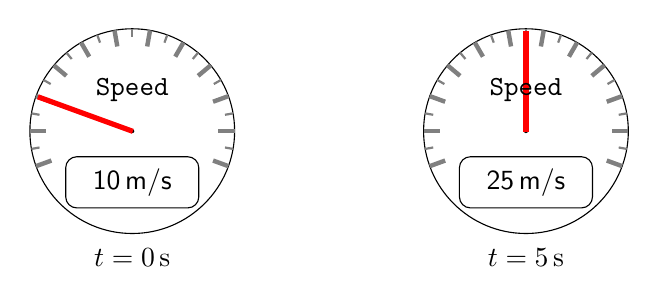
\begin{tikzpicture}
\uncover<2->{
\speedometer{(0,0)}{160}{10}
\node at (0,-1.6cm) {$t = \SI{0}{s}$};
}

\uncover<3->{
\speedometer{(5,0)}{90}{25}
\node at (5,-1.6cm) {$t = \SI{5}{s}$};
}
\end{tikzpicture}
\end{center}
\vspace{-3em}

{\color{red}
\begin{equation*}
    \uncover<4->{\bar{a} = \frac{\Delta v}{\Delta t}} 
    \uncover<5->{= \frac{\SI{25}{m/s} - \SI{10}{m/s}}{\SI{5}{s}}}
    \uncover<6->{= \frac{\SI{15}{m/s}}{\SI{5}{s}}}
    \uncover<7->{= \boxed{\SI{3}{m/s^2}}}
\end{equation*}
}
\end{frame}


\begin{frame}
\textit{Example.} Is the object below accelerating?
\vspace{-1em}

\begin{center}
\velocitytableI{0}{5}{0}{1}
\end{center}

\uncover<2->{\color{red}
Yes. The velocity is changing with time.
}
\end{frame}

\begin{frame}
\textit{Example. Find the average acceleration of the object below.}
\vspace{-1em}

\begin{center}
\velocitytableI{2}{-2}{5}{1}
\end{center}
\vspace{-1em}

\uncover<2->{\color{red}
Average acceleration is $\bar{a} = \SI{-2}{m/s^2}$. With each passing second, the velocity changes by \SI{-2}{m/s}.
}
\end{frame}

\section{position-time tables}

\begin{frame}
\textit{Example.} The motion map below shows positions of a particle at 1-second time intervals. Create a position-time table for the motion.
\vspace{-1.5em}

\begin{center}
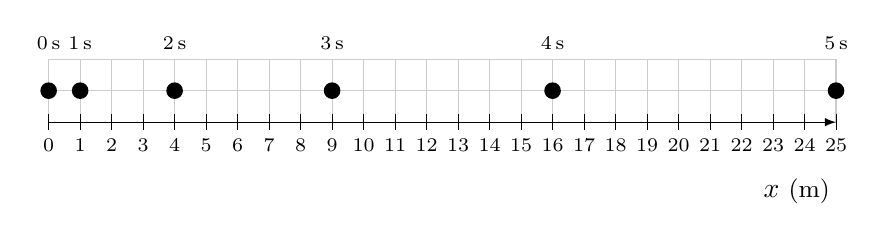
\begin{tikzpicture}[y=4mm,x=4mm]
    \draw[black!20,step=1] (0,0) grid (25,2);
    \node[above,opacity=0] at (0,2) {\scriptsize 0\,s};
    \foreach \x [evaluate=\x as \t using int(\x-2)] in {2,3,...,7}{
        \node<\x->[above] at ({(\x-2)^2},2) {\scriptsize \t\,s};
        \fill<\x-> ({(\x-2)^2},1) circle (3pt);
    }
    \foreach \x in {0,1,...,25} {
        \draw[ultra thin] (\x,-1mm) -- (\x,1mm) node[below=2mm] {\scriptsize $\x$};
    }
    \draw[->] (0,0) -- (25,0) node[below=6mm,pos=0.95] {$x$ {\small (m)}};
\end{tikzpicture}
\vspace{-2em}

\uncover<8->{\small
\def\arraystretch{1.2}
\begin{tabular}{|c|c|}
    \hline
    \thead{Time (s)} & \thead{Position (m)} \\ \hline
    0 & \uncover<9->{\textcolor{red}{0}} \\ \hline
    1 & \uncover<10->{\textcolor{red}{1}} \\ \hline
    2 & \uncover<11->{\textcolor{red}{4}} \\ \hline
    3 & \uncover<12->{\textcolor{red}{9}} \\ \hline
    4 & \uncover<13->{\textcolor{red}{16}} \\ \hline
    5 & \uncover<14->{\textcolor{red}{25}} \\ \hline
\end{tabular}}
\end{center}
\end{frame}

\begin{frame}
\textit{Example.} Is the object below traveling with constant velocity?
\vspace{-1em}

\begin{center}
\begin{tabular}{|c|c|}
    \hline
    \thead{Time (s)} & \thead{Position (m)} \\ \hline
    0 & 0 \\ \hline
    1 & 1 \\ \hline
    2 & 4 \\ \hline
    3 & 9 \\ \hline
    4 & 16 \\ \hline
    5 & 25 \\ \hline
\end{tabular}

\begin{tikzpicture}[overlay]
    \node<2->[red,left] at (-1.9cm,3.6cm) {$\Delta t = \SI{1}{s}$ \{ };
    \node<3->[red,left] at (-1.9cm,2.99cm) {$\Delta t = \SI{1}{s}$ \{ };
    \node<4->[red,left] at (-1.9cm,2.38cm) {$\Delta t = \SI{1}{s}$ \{ };
    \node<5->[red,left] at (-1.9cm,1.77cm) {$\Delta t = \SI{1}{s}$ \{ };
    \node<6->[red,left] at (-1.9cm,1.16cm) {$\Delta t = \SI{1}{s}$ \{ };
    \node<7->[red,right] at (1.9cm,3.6cm) {\} $\Delta x = \SI{1}{m}$};
    \node<8->[red,right] at (1.9cm,2.99cm) {\} $\Delta x = \SI{3}{m}$};
    \node<9->[red,right] at (1.9cm,2.38cm) {\} $\Delta x = \SI{5}{m}$};
    \node<10->[red,right] at (1.9cm,1.77cm) {\} $\Delta x = \SI{7}{m}$};
    \node<11->[red,right] at (1.9cm,1.16cm) {\} $\Delta x = \SI{9}{m}$};
\end{tikzpicture}
\end{center}
\vspace{-2.5em}


\textcolor{red}{
\uncover<12->{Average velocity is $\bar{v} = \frac{\Delta x}{\Delta t}$.}
\uncover<13->{The displacements $\Delta x$ are NOT constant.}
\uncover<14->{So, the object's velocity is NOT constant.}
}

\end{frame}


\section{velocity vs time graphs}

{\setbeamercolor{background canvas}{bg = black!10}
\againframe<4>{E3ngE}
\againframe<7>{E3ngE}
}

\begin{frame}
\textit{Example.} Sketch a velocity-vs-time graph of the scooter from the previous problem.
\vspace{-1em}

\begin{center}
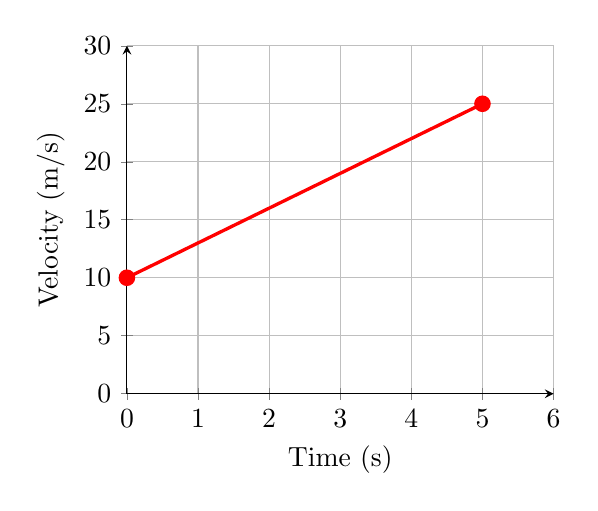
\begin{tikzpicture}
    \begin{axis}[height=6cm,
    width=7cm,
    ylabel={Velocity (m/s)},
    xlabel={Time (s)},
    axis lines=left,
    ymin=0,ymax=30,
    xmin=0,xmax=6,
    ytick={0,5,...,30},
    xtick={0,1,...,6},
    clip=false,
    grid=both,
    ]
    \fill<2->[red] (0,10) circle (3pt);
    \fill<3->[red] (5,25) circle (3pt);
    \draw<4->[very thick,red] (0,10) -- (5,25);
    \end{axis}
\end{tikzpicture}
\end{center}
\end{frame}

\begin{frame}
\textit{Example.} What physical quantity does the slope of the line below represent? 
\uncover<7->{\textcolor{red}{\textit{Answer:} avg.\,acceleration}}
\vspace{-1em}

\begin{center}
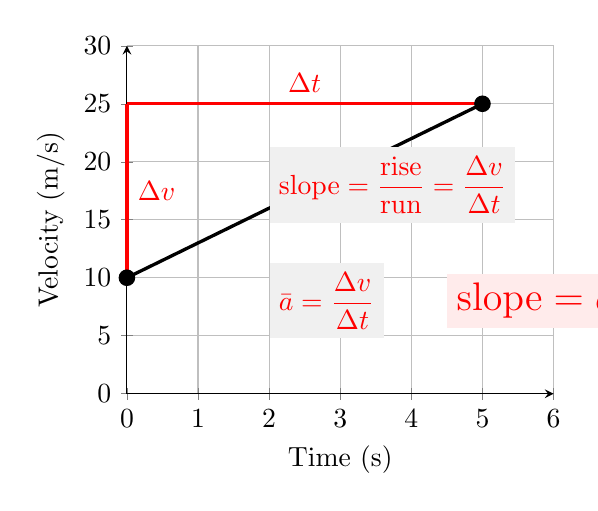
\begin{tikzpicture}
    \begin{axis}[height=6cm,
    width=7cm,
    ylabel={Velocity (m/s)},
    xlabel={Time (s)},
    axis lines=left,
    ymin=0,ymax=30,
    xmin=0,xmax=6,
    ytick={0,5,...,30},
    xtick={0,1,...,6},
    clip=false,
    grid=both,
    ]
    \draw<2->[red,very thick] (0,10) -- (0,25) node[pos=0.5,right] {$\Delta v$};
    \draw<3->[red,very thick] (0,25) -- (5,25) node[pos=0.5,above] {$\Delta t$};
    \fill (0,10) circle (3pt);
    \fill (5,25) circle (3pt);
    \draw[very thick] (0,10) -- (5,25);
    \node<4->[red,fill=black!6,overlay,right] at (2,18) {$\displaystyle \text{slope} = \frac{\text{rise}}{\text{run}} = \frac{\Delta v}{\Delta t}$};
    \node<5->[red,fill=black!6,overlay,right] at (2,8) {$\displaystyle \bar{a} = \frac{\Delta v}{\Delta t}$};
    \node<6->[red,fill=red!8,overlay,right] at (4.5,8) {\Large $\displaystyle \text{slope} = \bar{a}$};
    \end{axis}
\end{tikzpicture}
\end{center}
\end{frame}



\begin{frame}
\textit{Example.} Calculate the average acceleration of the object below.
\vspace{1ex}

\pgfdeclarelayer{foreground}
\pgfsetlayers{background,main,foreground}
\begin{tikzpicture}
    \begin{axis}[height=6cm,
    width=7cm,
    ylabel={Velocity (m/s)},
    xlabel={Time (s)},
    axis lines=left,
    ymin=0,ymax=30,
    xmin=0,xmax=6,
    ytick={0,5,...,30},
    xtick={0,1,...,6},
    clip=true,
    grid=both,
    ]
    \addplot[very thick,domain=0:6] {40 - 5*x};
    \begin{pgfonlayer}{foreground}
        \draw<3->[thick,densely dashed] (2,30) -- (2,10) node[red,left,pos=0.5] {$\Delta v$};
        \draw<3->[thick,densely dashed] (2,10) -- (6,10) node[red,below,pos=0.5] {$\Delta t$};
        \fill<2->[red] (2,30) circle (3pt) node[shift={(0,0.7cm)},align=center] {\small $(t_1,v_1)$\\ \small $(2,30)$};
        \fill<2->[red] (6,10) circle (3pt) node[shift={(0,-0.7cm)},align=center] {\small $(6,10)$\\ \small $(t_2,v_2)$};
        \node<4->[red,right] at (3.5,34) {$\displaystyle \bar{a} = \text{slope} = \frac{\Delta v}{\Delta t} = \frac{v_2 - v_1}{t_2 - t_1}$};
        \node<5->[red,right] at (4,23) {$\displaystyle \bar{a} = \frac{10\,\text{\footnotesize m/s} - 30\,\text{\footnotesize m/s}}{6\,\text{\footnotesize s} - 2\,\text{\footnotesize s}}$};
        \node<6->[red,right,fill=red!8] at (6.3,14) {$\boxed{\bar{a} = \SI{-5}{m/s^2}}$};
    \end{pgfonlayer}
    \end{axis}
\end{tikzpicture}
\end{frame}

\section{position vs time graphs}

\begin{frame}
\textit{Example.} Using the table, graph position vs time.
\vspace{-1em}

\begin{center}
\begin{minipage}[t]{2.9cm}
\vspace{0pt}%
\def\arraystretch{1.25}
\begin{tabular}{|c|c|}
    \hline
    \thead{$t$ (s)} & \thead{$x$ (m)} \\ \hline
    0 & 0 \\ \hline
    1 & 1 \\ \hline
    2 & 4 \\ \hline
    3 & 9 \\ \hline
    4 & 16 \\ \hline
    5 & 25 \\ \hline
\end{tabular}
\end{minipage}%
\begin{minipage}[t]{7cm}
\vspace{0pt}%
\centering
\begin{tikzpicture}
    \begin{axis}[height=6.2cm,width=6.6cm,
        ylabel={\small Position (m)},
        xlabel={\small Time (s)},
        ymin=0,ymax=25,
        xmin=0,xmax=5,
        ytick={0,5,...,25},
        xtick={0,1,...,5},
        grid=both,
        axis lines=left,
        clip=false,
        major grid style={thick, draw=black!60},
        minor grid style={thin, draw=gray!30},
        minor y tick num=4,
        minor x tick num=4,
    ]
    \only<2->{
            \addplot[only marks,mark=*,red] coordinates{(0,0)(1,1)(2,4)(3,9)(4,16)(5,25)};
    }
    \only<3->{
            \addplot[red,smooth,domain=0:5,thick] {x^2};
        }   
    \end{axis}
\end{tikzpicture}
\end{minipage}
\end{center}
\end{frame}

\begin{frame}
\textit{Example.} What is the shape of the position vs time graph for an object undergoing constant acceleration? Is it linear?
\vspace{-1em}

\begin{minipage}[t]{4.2cm}
\vspace{0pt}%
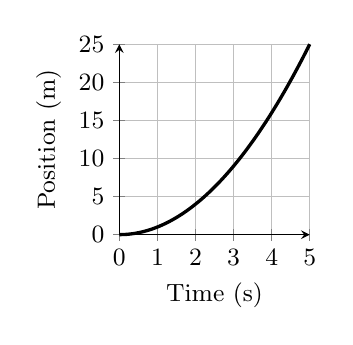
\begin{tikzpicture}
    \small 
    \begin{axis}[height=4cm,width=4cm,
        ylabel={Position (m)},
        xlabel={Time (s)},
        ymin=0,ymax=25,
        xmin=0,xmax=5,
        ytick={0,5,...,25},
        xtick={0,1,...,5},
        grid=both,
        axis lines=left,
        clip=false,
    ]
    \addplot[smooth,domain=0:5,very thick] {x^2};
    \end{axis}
\end{tikzpicture}
\end{minipage}%
\pause
\begin{minipage}[t]{5.6cm}
\vspace{0pt}%
\small\color{red}
\begin{itemize}[<+->]
    \setlength{\leftmargini}{1.2em} % Reduces left indent to save width
    \setlength{\itemsep}{3pt}       % Keeps spacing between points compact
    \item The shape is not linear.
    \item Position increases \textbf{\underline{quadratically}} with time.
    \item The shape of the $x$ vs $t$ graph is quadratic.
    \item A quadratic shape is the shape of a parabola.
\end{itemize}
\end{minipage}

\begin{tikzpicture}[overlay,shift={(6.5cm,-1cm)},y=1.2cm]
\draw<6->[domain=-1:1,red,very thick] plot({\x,\x*\x});
\end{tikzpicture}
\end{frame}


\section{Galileo's law of odd numbers}

\begin{frame}
\vspace{-8mm}
\begin{center}
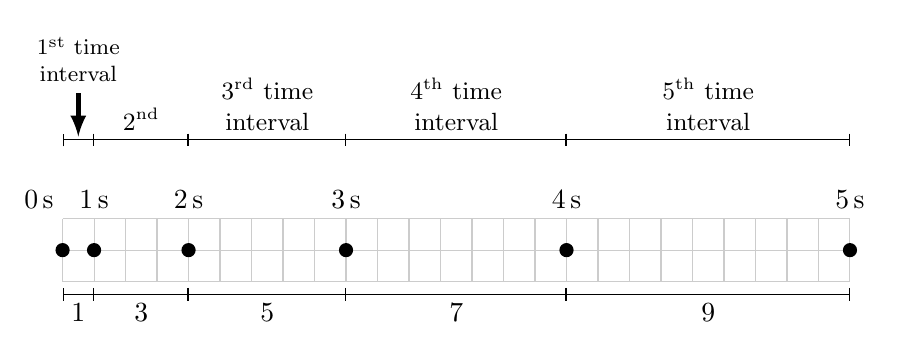
\begin{tikzpicture}[y=4mm,x=4mm]
    \draw[black!20,step=1] (0,0) grid (25,2);
        \foreach \x in {2,3,...,7}{
        \fill<\x-> ({(\x-2)^2},1) circle (0.9mm);
    }
    \uncover<8->{
        \node[above,shift={(-3mm,0)},overlay] at (0,2) {$\SI{0}{s}$};
        \foreach \x in {1,2,...,5}{
            \node[above] at (\x*\x,2) {$\SI{\x}{s}$};
        }
    }
    
    \uncover<9->{
        \draw[|-|] (0,4.5) -- ++(1,0);
        \draw[ultra thick,<-] (0.5,4.6) -- (0.5,6) node[above,align=center,font=\footnotesize] { 1\textsuperscript{st} time\\interval};
    }
    \uncover<10->{
        \draw[-|] (1,4.5) -- ++(3,0) node[above,pos=0.5,font=\small] {2\textsuperscript{nd}};
    }
    \uncover<11->{
        \draw[-|] (4,4.5) -- ++(5,0) node[above,pos=0.5,font=\small,align=center] {3\textsuperscript{rd} time\\interval};
    }
    \uncover<12->{
        \draw[-|] (9,4.5) -- ++(7,0) node[above,pos=0.5,font=\small,align=center] {4\textsuperscript{th} time\\interval};
    }
    \uncover<13->{
        \draw[-|] (16,4.5) -- ++(9,0) node[above,pos=0.5,font=\small,align=center] {5\textsuperscript{th} time\\interval};
    }
    
    \uncover<14->{
        \draw[|-|] (0,-0.4) -- ++(1,0) node[below,pos=0.5] {1};
    }
    \uncover<15->{
        \draw[-|] (1,-0.4) -- ++(3,0) node[below,pos=0.5] {3};
    }
    \uncover<16->{
        \draw[-|] (4,-0.4) -- ++(5,0) node[below,pos=0.5] {5};
    }
    \uncover<17->{
        \draw[-|] (9,-0.4) -- ++(7,0) node[below,pos=0.5] {7};
    }
    \uncover<18->{
        \draw[-|] (16,-0.4) -- ++(9,0) node[below,pos=0.5] {9};
    }
\end{tikzpicture}
\end{center}

\uncover<19->{\textbf{\gls{Galileo's law of odd numbers}}:} \uncover<20->{\glsdesc{Galileo's law of odd numbers}}
\end{frame}


\end{document}

